%%%%%%%%%%%%%%%%%%%%%%%%%%%%%%%%%%%%%%%%%%%%%%%%%%%%%%%%%%%%%%%%%%%%%%%%%%%%%%%%%%%%%%%
%%%%%%%%%%%%%%%%%%%%%%%%%%%%%%%%%%%%%%%%%%%%%%%%%%%%%%%%%%%%%%%%%%%%%%%%%%%%%%%%%%%%%%%
% 
% This top part of the document is called the 'preamble'.  Modify it with caution!
%
% The real document starts below where it says 'The main document starts here'.

\documentclass[12pt]{article}

\usepackage{amssymb,amsmath,amsthm}
\usepackage[top=1in, bottom=1in, left=1.25in, right=1.25in]{geometry}
\usepackage{fancyhdr}
\usepackage{graphicx}
\usepackage{enumerate}
\usepackage{listings}
\usepackage{verbatim}
\usepackage{xcolor}

% Comment the following line to use TeX's default font of Computer Modern.
\usepackage{times,txfonts}


\definecolor{codegreen}{rgb}{0,0.6,0}
\definecolor{codegray}{rgb}{0.5,0.5,0.5}
\definecolor{codepurple}{rgb}{0.58,0,0.82}
\definecolor{backcolour}{rgb}{0.95,0.95,0.92}

\lstdefinestyle{mystyle}{
    backgroundcolor=\color{backcolour},   
    commentstyle=\color{codegreen},
    keywordstyle=\color{magenta},
    numberstyle=\tiny\color{codegray},
    stringstyle=\color{codepurple},
    basicstyle=\ttfamily\footnotesize,
    breakatwhitespace=false,         
    breaklines=true,                 
    captionpos=b,                    
    keepspaces=true,                 
    numbers=left,                    
    numbersep=5pt,                  
    showspaces=false,                
    showstringspaces=false,
    showtabs=false,                  
    tabsize=2
}

\lstset{style=mystyle}

\newtheoremstyle{homework}% name of the style to be used
  {18pt}% measure of space to leave above the theorem. E.g.: 3pt
  {12pt}% measure of space to leave below the theorem. E.g.: 3pt
  {}% name of font to use in the body of the theorem
  {}% measure of space to indent
  {\bfseries}% name of head font
  {:}% punctuation between head and body
  {2ex}% space after theorem head; " " = normal interword space
  {}% Manually specify head
\theoremstyle{homework} 

% Set up an Exercise environment and a Solution label.
\newtheorem*{exercisecore}{\@currentlabel}
\newenvironment{exercise}[1]
{\def\@currentlabel{#1}\exercisecore}
{\endexercisecore}

\newcommand{\localhead}[1]{\par\smallskip\noindent\textbf{#1}\nobreak\\}%
\newcommand\solution{\localhead{Solution:}}



% \newcommand{includematlab}[1]{\verbatiminput{#1}}

%%%%%%%%%%%%%%%%%%%%%%%%%%%%%%%%%%%%%%%%%%%%%%%%%%%%%%%%%%%%%%%%%%%%%%%%
%
% Stuff for getting the name/document date/title across the header
\makeatletter
\RequirePackage{fancyhdr}
\pagestyle{fancy}
\fancyfoot[C]{\ifnum \value{page} > 1\relax\thepage\fi}
\fancyhead[L]{\ifx\@doclabel\@empty\else\@doclabel\fi}
\fancyhead[C]{\ifx\@docdate\@empty\else\@docdate\fi}
\fancyhead[R]{\ifx\@docauthor\@empty\else\@docauthor\fi}
\headheight 15pt

\def\doclabel#1{\gdef\@doclabel{#1}}
\doclabel{Use {\tt\textbackslash doclabel\{MY LABEL\}}.}
\def\docdate#1{\gdef\@docdate{#1}}
\docdate{Use {\tt\textbackslash docdate\{MY DATE\}}.}
\def\docauthor#1{\gdef\@docauthor{#1}}
\docauthor{Use {\tt\textbackslash docauthor\{MY NAME\}}.}
\makeatother

%% General formatting parameters
\parindent 0pt
\parskip 12pt plus 1pt

% Shortcuts for blackboard bold number sets (reals, integers, etc.)
\newcommand{\Reals}{\ensuremath{\mathbb R}}
\newcommand{\Nats}{\ensuremath{\mathbb N}}
\newcommand{\Ints}{\ensuremath{\mathbb Z}}
\newcommand{\Rats}{\ensuremath{\mathbb Q}}
\newcommand{\Cplx}{\ensuremath{\mathbb C}}
%% Some equivalents that some people may prefer.
\let\RR\Reals
\let\NN\Nats
\let\II\Ints
\let\CC\Cplx

%%%%%%%%%%%%%%%%%%%%%%%%%%%%%%%%%%%%%%%%%%%%%%%%%%%%%%%%%%%%%%%%%%%%%%%%%%%%%%%%%%%%%%%
%%%%%%%%%%%%%%%%%%%%%%%%%%%%%%%%%%%%%%%%%%%%%%%%%%%%%%%%%%%%%%%%%%%%%%%%%%%%%%%%%%%%%%%
% 
% The main document start here.

% The following commands set up the material that appears in the header.
\doclabel{Math 426: Homework 2}
\docauthor{Andrew Player}
\docdate{September 9, 2020}

\newcommand{\vv}{\mathbf{v}}
\begin{document}

\begin{exercise}{DM 1}
Write a small Matlab function \texttt{largest(a,b)} that
returns the largest of the two values.  Test that your function
works by computing \texttt{largest(1,2)}, \texttt{largest(0,-1)}
and \texttt{largest(5,5)}.
\end{exercise}
\solution

\begin{lstlisting}[language=Matlab]
function c = largest(a, b)
    if (a > b)
        c = a;
        return
    end
    c = b;
end
\end{lstlisting}

Output:
\begin{lstlisting}[language=Matlab]
	>> largest(1,2)

	ans =
	
		 2
	
	>> largest(0,-1)
	
	ans =
	
		 0
	
	>> largest(5,5)
	
	ans =
	
		 5
\end{lstlisting}

\begin{exercise}{DM 2} Write a small Matlab function \texttt{nextprime(x)} 
that takes a positive integer argument and returns the smallest 
prime number at least as large as \texttt{x}.  Your function should
use a \texttt{while} loop and take advantage of the \texttt{isprime}
function in Matlab.  Test that your function works by computing 
\texttt{nextprime(5)}, \texttt{nextprime(6)}, \texttt{nextprime(-1)}
and \texttt{nextprime(100)}.
\end{exercise}
\solution

\begin{lstlisting}[language=Matlab]
function y = nextprime(x)
    %isprime does not work for negative numbers
    %so we just return 2, the first prime number.
    if(x < 2)
        y = 2;
        return
    end
    while ~isprime(x)
        x = x + 1;
    end
    y = x;
end
\end{lstlisting}

Output:
\begin{lstlisting}[language=Matlab]
	>> nextprime(5)

	ans =
	
		 5
	
	>> nextprime(6)
	
	ans =
	
		 7
	
	>> nextprime(-1)
	
	ans =
	
		 2
	
	>> nextprime(100)
	
	ans =
	
	   101
\end{lstlisting}

\begin{exercise}{DM 3} Define a sequence of numbers by $x_1=1$ and $x_{k+1}=\frac{1}{2}x_{k} + 1$.  Write a Matlab function \texttt{buildseq(N)} that returns an array
with the first \texttt{N} elements of the sequence in it.  For example,
\texttt{buildseq(2)} should return $[1,1.5]$.  Test that your function
works by computing the first four sequence elements by hand, and then
verifying that your function computes them correctly.  You may wish 
to take advantage of the Matlab command \texttt{zeros}.
\end{exercise}
\solution

\begin{lstlisting}[language=Matlab]
function x = buildseq(n)
    x = [1:n];
    for i = 2:n
        x(i) = (1/2)*x(i-1)+1;
    end
end
\end{lstlisting}
\begin{verbatim}




Expected Output (by hand):

buildseq(4) =
	x(1) = (1/2)*x(1-1)+1                 = 1
	x(2) = (1/2)*x(2-1)+1 = 1/2 + 1       = 1.5
	x(3) = (1/2)*x(3-1)+1 = 1/2(1.5) + 1  = 1.75
	x(4) = (1/2)*x(4-1)+1 = 1/2(1.75) + 1 = 1.875

\end{verbatim}
Output:
\begin{lstlisting}[language=Matlab]
	>> buildseq(4)

	ans =
	
	  Columns 1 through 2
	
	   1.000000000000000   1.500000000000000
	
	  Columns 3 through 4
	
	   1.750000000000000   1.875000000000000
\end{lstlisting}

\begin{exercise}{DM 4}
Write a function \texttt{HW2bisect} that does the following:
\begin{enumerate}
	\item Takes the following input:
	\begin{itemize}
		\item \texttt{f}, the name of a function
		\item Numbers \texttt{a} and \texttt{b} that (supposedly) bound an interval containing a root of \texttt{f}.
		\item \texttt{delta}, a number determining the accuracy of the sollution.
	\end{itemize}
\end{enumerate}
Your function should approximate a root of $f$ in the interval $[a,b]$ by 
bisection.  The approximation $x$ should be within $\delta$ of a root

The function should return:
\begin{enumerate}
	\item \texttt{x}, the approximate root
	\item A $n\times 2$ matrix \texttt{history} that contains
	a list of the interval endpoints at each stage, starting with the
	initial guess provided.
	\begin{equation}
	\mathtt{hist} = \begin{pmatrix} a_0 & b_0 \\
	a_1 & b_1 \\
	\vdots & \vdots \\
	a_n & b_n \\
	\end{pmatrix}
	\end{equation}
\end{enumerate}

Your function should have help and should produce error messages appropriately when the function fails.

Test your function works by applying it to the function $f(x)=x^2-4$ with starting interval $[0,5]$.
\end{exercise}

\solution

\begin{lstlisting}[language=Matlab]
function [x, history] = HW2bisect(f, a, b, delta)
    
    %Nx2 Array containing the intervals from each step 
    history = [];
    
    %Root approximation
    x = 0;
    
    %If the function does not have opposite signs along the interval
    %the function algorithm will not work so we throw an error and return
    if ~(f(a) > 0 && f(b) < 0) && ~(f(a) < 0 && f(b) > 0)
        disp("ERROR: Function does not have opposite signs at: ")
        disp([a,b])
        return
    end
    
    %Main loop for the algorithm
    while(true)
        
        %Bisection step
        c = (a + b) / 2;

        %Every iteration adds a row to history with the current interval
        history = [history ;[a, b]];

        %If f(c) == 0 or it is less then or equal to the tolerance
        %we have found the root and can return
        if f(c) == 0
            x = c;
            return
        elseif abs(f(c)) <= delta
           x = c;
           return
        end

        %Maintain opposite signs
        if sign(f(a)) == sign(f(c))
           a = c;
        else
           b = c;
        end
    end
end
\end{lstlisting}

Output:
\begin{lstlisting}[language=Matlab]
	>> func = @(x) (x^2 - 4);
	>> [x, history] = HW2bisect(func, 0, 5, 1e-8);
	>> x
	
	x =
	
	   2.000000001862645
	
	>> history
	
	history =
	
                     0   5.000000000000000
                     0   2.500000000000000
	   1.250000000000000   2.500000000000000
	   1.875000000000000   2.500000000000000
	   1.875000000000000   2.187500000000000
	   1.875000000000000   2.031250000000000
	   1.953125000000000   2.031250000000000
	   1.992187500000000   2.031250000000000
	   1.992187500000000   2.011718750000000
	   1.992187500000000   2.001953125000000
	   1.997070312500000   2.001953125000000
	   1.999511718750000   2.001953125000000
	   1.999511718750000   2.000732421875000
	   1.999511718750000   2.000122070312500
	   1.999816894531250   2.000122070312500
	   1.999969482421875   2.000122070312500
	   1.999969482421875   2.000045776367188
	   1.999969482421875   2.000007629394531
	   1.999988555908203   2.000007629394531
	   1.999998092651367   2.000007629394531
	   1.999998092651367   2.000002861022949
	   1.999998092651367   2.000000476837158
	   1.999999284744263   2.000000476837158
	   1.999999880790710   2.000000476837158
	   1.999999880790710   2.000000178813934
	   1.999999880790710   2.000000029802322
	   1.999999955296516   2.000000029802322
	   1.999999992549419   2.000000029802322
	   1.999999992549419   2.000000011175871
\end{lstlisting}

\begin{exercise}{Chapter 4: 2(a)} 
[You should use the code developed in the previous problem.]
\end{exercise}
Output:
\begin{lstlisting}[language=Matlab]
	>> func = @(x) ((5-x)*exp(x)-5);
	>> [x, history] = HW2bisect(func, 4, 5, 1e-6);
	>> x
	
	x =
	
	   4.965114235877991
	
	>> history
	
	history =
	
	   4.000000000000000   5.000000000000000
	   4.500000000000000   5.000000000000000
	   4.750000000000000   5.000000000000000
	   4.875000000000000   5.000000000000000
	   4.937500000000000   5.000000000000000
	   4.937500000000000   4.968750000000000
	   4.953125000000000   4.968750000000000
	   4.960937500000000   4.968750000000000
	   4.964843750000000   4.968750000000000
	   4.964843750000000   4.966796875000000
	   4.964843750000000   4.965820312500000
	   4.964843750000000   4.965332031250000
	   4.965087890625000   4.965332031250000
	   4.965087890625000   4.965209960937500
	   4.965087890625000   4.965148925781250
	   4.965087890625000   4.965118408203125
	   4.965103149414062   4.965118408203125
	   4.965110778808594   4.965118408203125
	   4.965110778808594   4.965114593505859
	   4.965112686157227   4.965114593505859
	   4.965113639831543   4.965114593505859
	   4.965114116668701   4.965114593505859
	   4.965114116668701   4.965114355087280
\end{lstlisting}
\begin{verbatim}
Guess and Explination for 10^-12
	
It appears to take around 4 iterations for each digit of accuracy 
(given that it took 23 to get 6 digits of accuracy). So it should 
take around 3*6 = 24 more iterations to get 10-12 digits of accuracy. 
\end{verbatim}

\begin{exercise}{Chapter 4: 18}
Produce a set of four plots of the first four Taylor polynomials of
the function $f(x)=e^{1-x^2}$, expanded around the point $x=1$.
\end{exercise}
\begin{verbatim}
Working them out: 

1st: = e^(1-1^2) = 1
2nd: 1st + (f'(a)(x-a)) = -2(1)(x-1) = 1 - 2x + 2
3rd: 1st + 2nd + (f''(a)/2!)(x-a)^2 = 1 - 2(x-1) + (x-1)^2
4th: 1st + 2nd + 3rd + (f'''(a)/3!)(x-a)^3 = d^3/dx^3(e^(1 - x^2)) 
   = 1 - 2(x-1) + (x-1)^2 + (2/3)(x-1)^3
\end{verbatim}
Plots:
\newline
1st Polynomial:
\newline
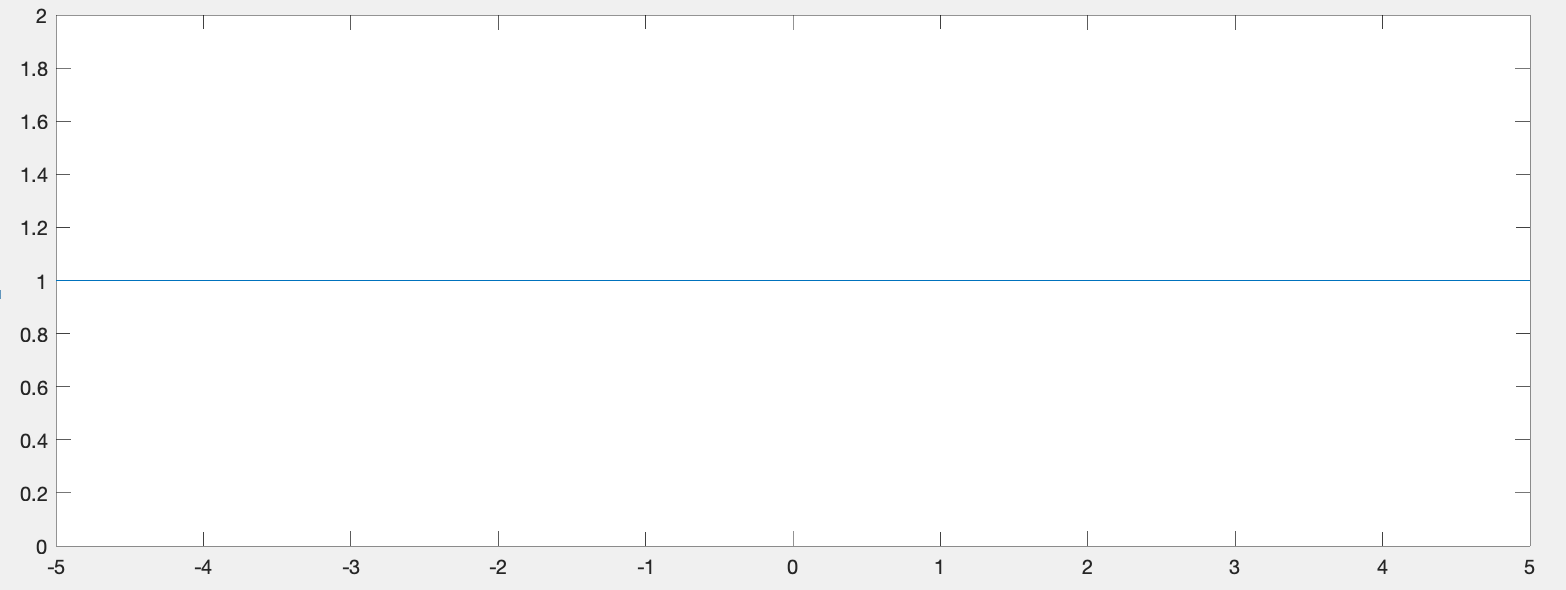
\includegraphics[scale=0.5]{1st.png}
\newline
2nd Polynomial:
\newline
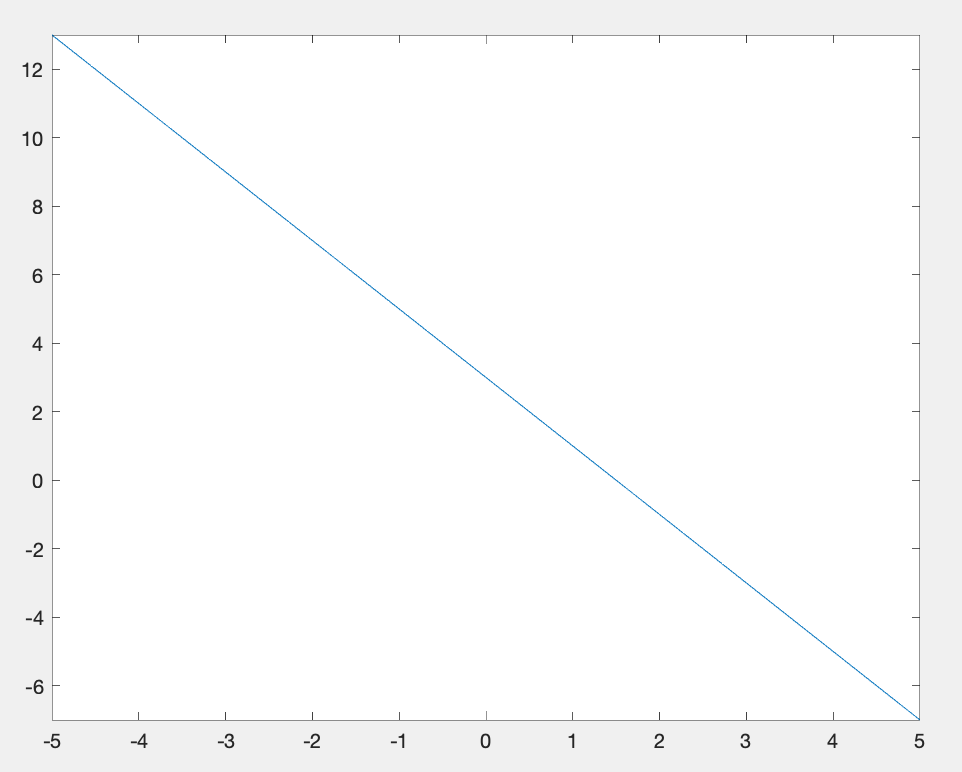
\includegraphics[scale=0.5]{2nd.png}
\newline
3rd Polynomial:
\newline
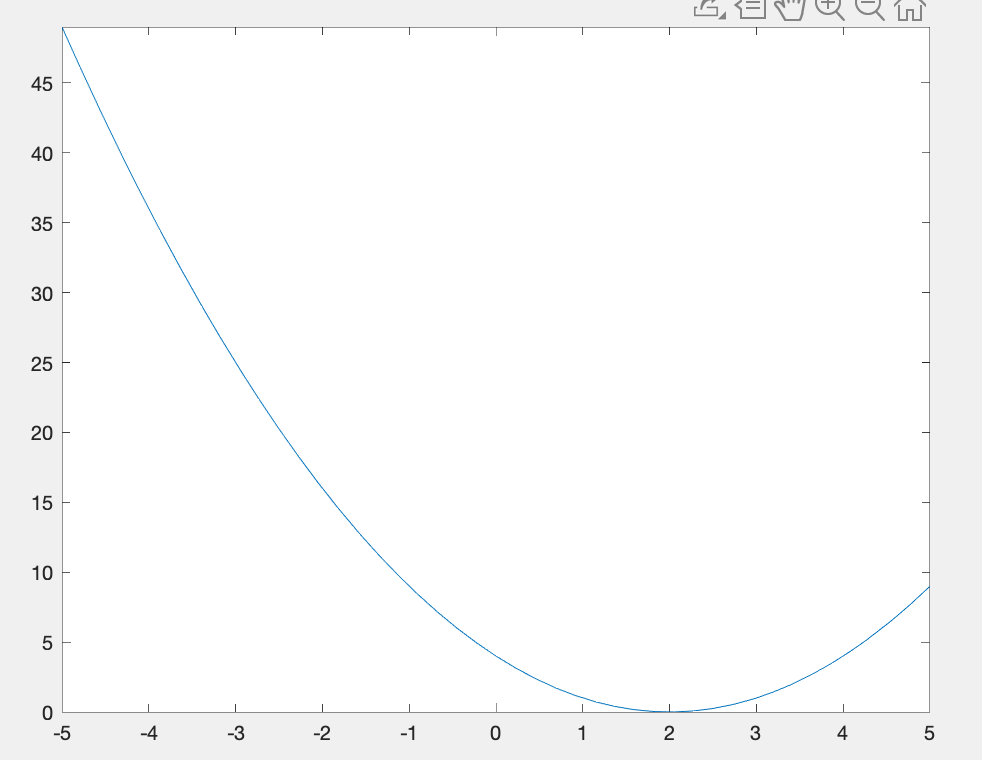
\includegraphics[scale=0.5]{3rd.png}
\newline
4th Polynomial:
\newline
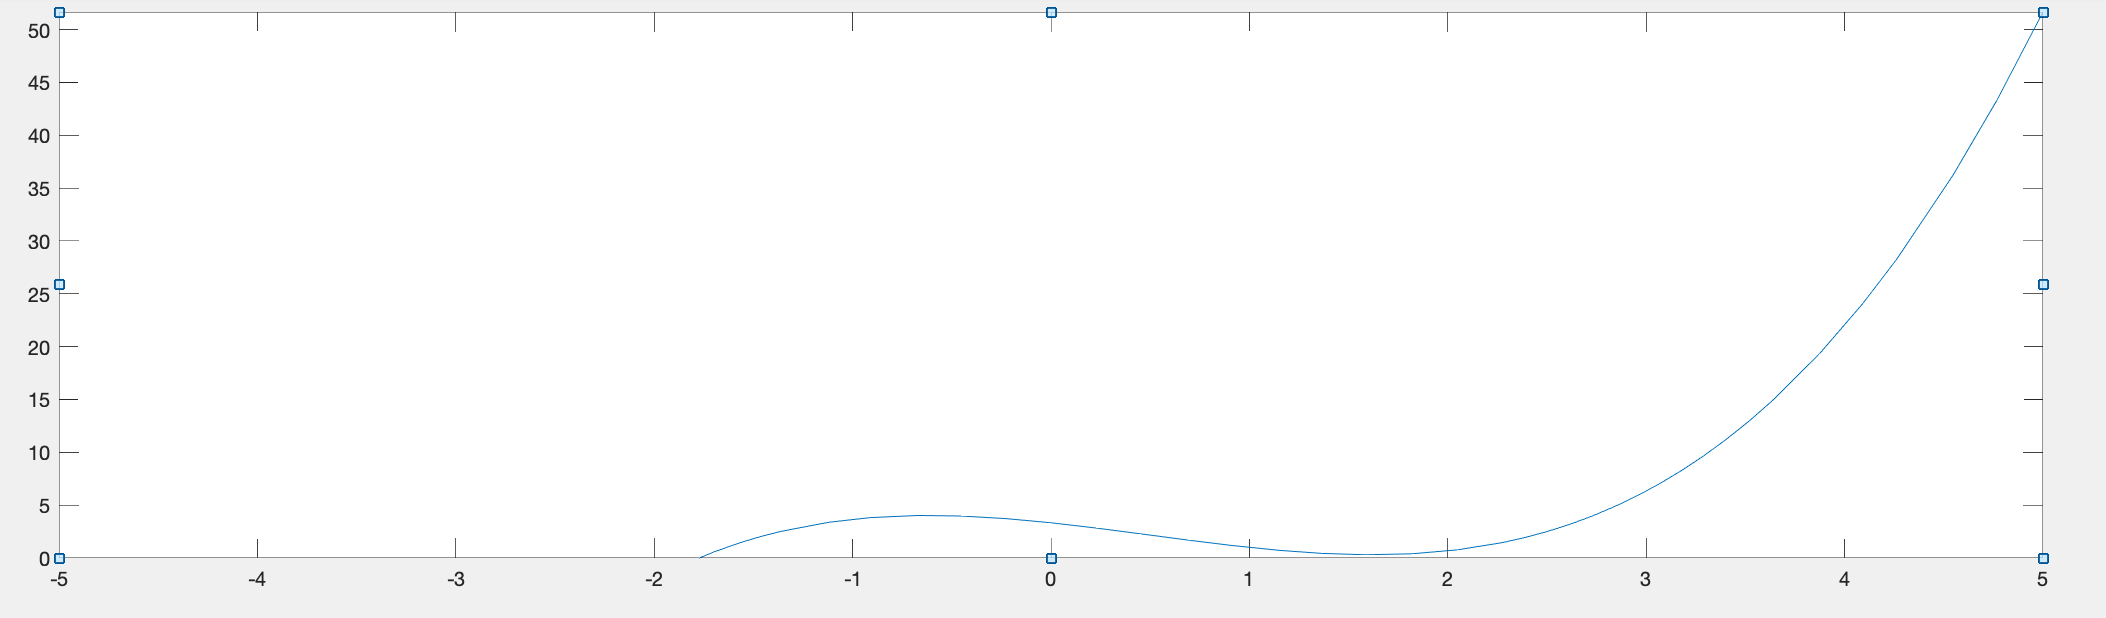
\includegraphics[scale=0.5]{4th.png}

\end{document}